\subsection{Qualitative data}

Everyone now thought the app was good and easy to use. The interview answers of what the coaches said about the app were clustered into areas of Learning, figure \ref{fig:learning}, Interaction Design, figure \ref{fig:interactiondesign}, and Service Design, figure \ref{fig:servicedesign}.

\begin{figure}[h]
    \centering
    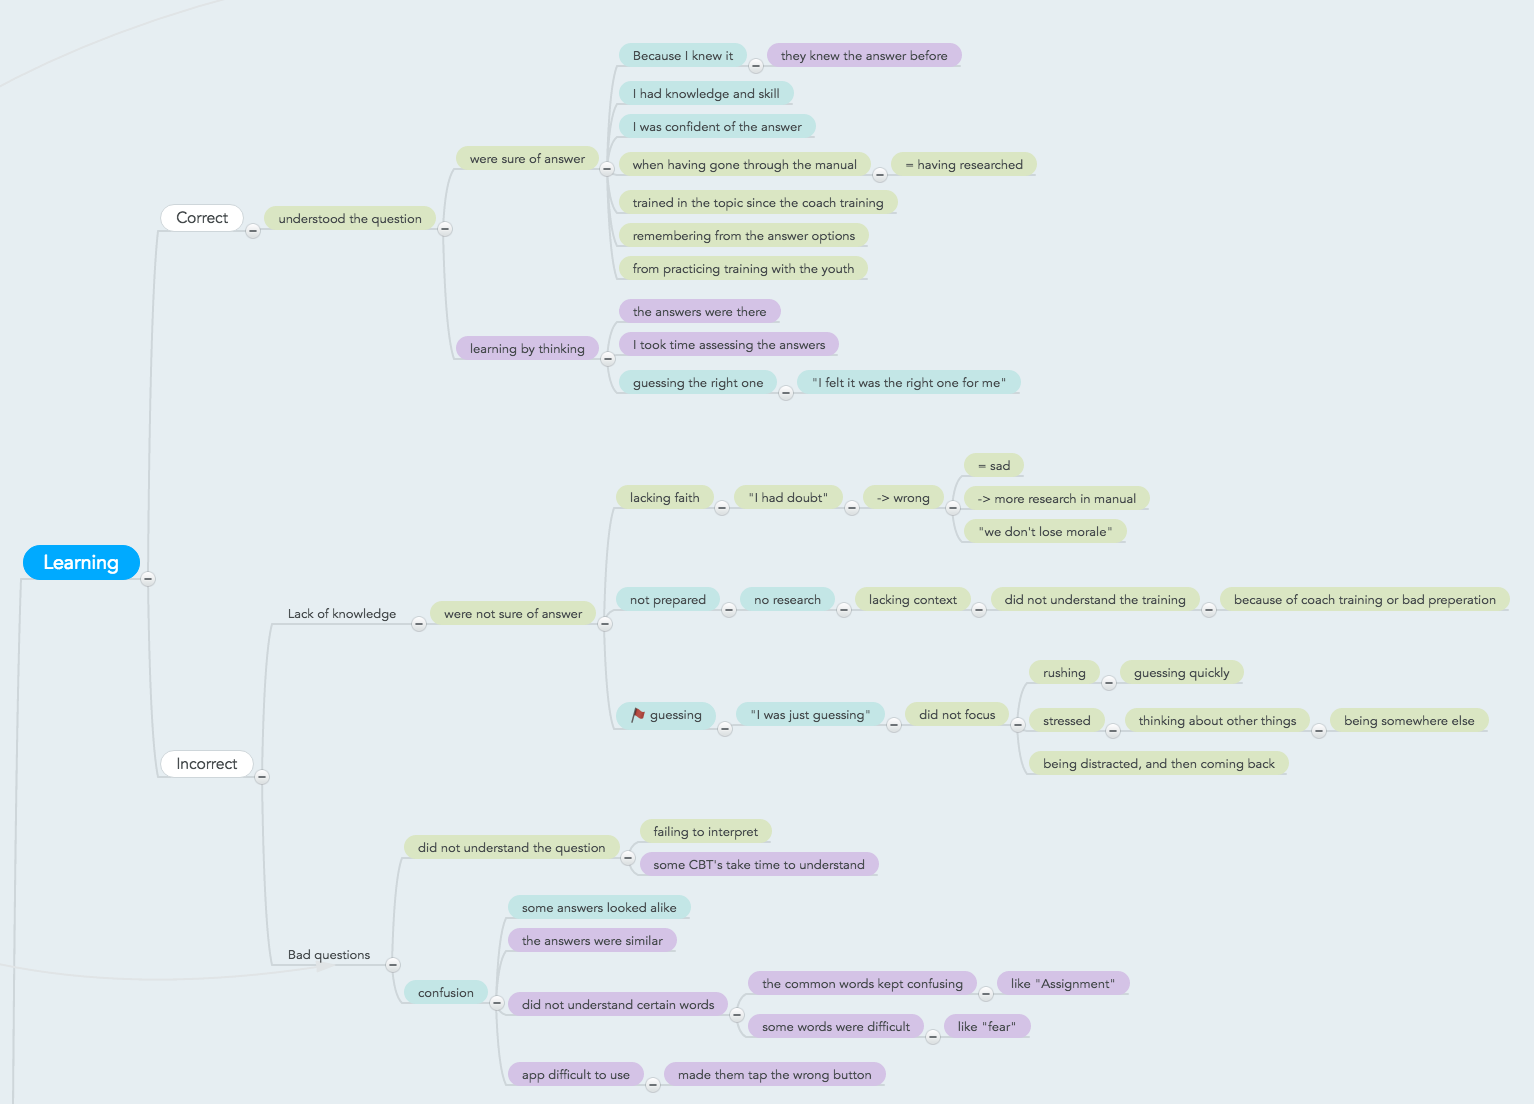
\includegraphics[width=1.0\textwidth]{iteration4qualitative_learning.png}
    \caption{Coach comments regarding learning}
    \label{fig:learning}
\end{figure}

\begin{figure}[h]
    \centering
    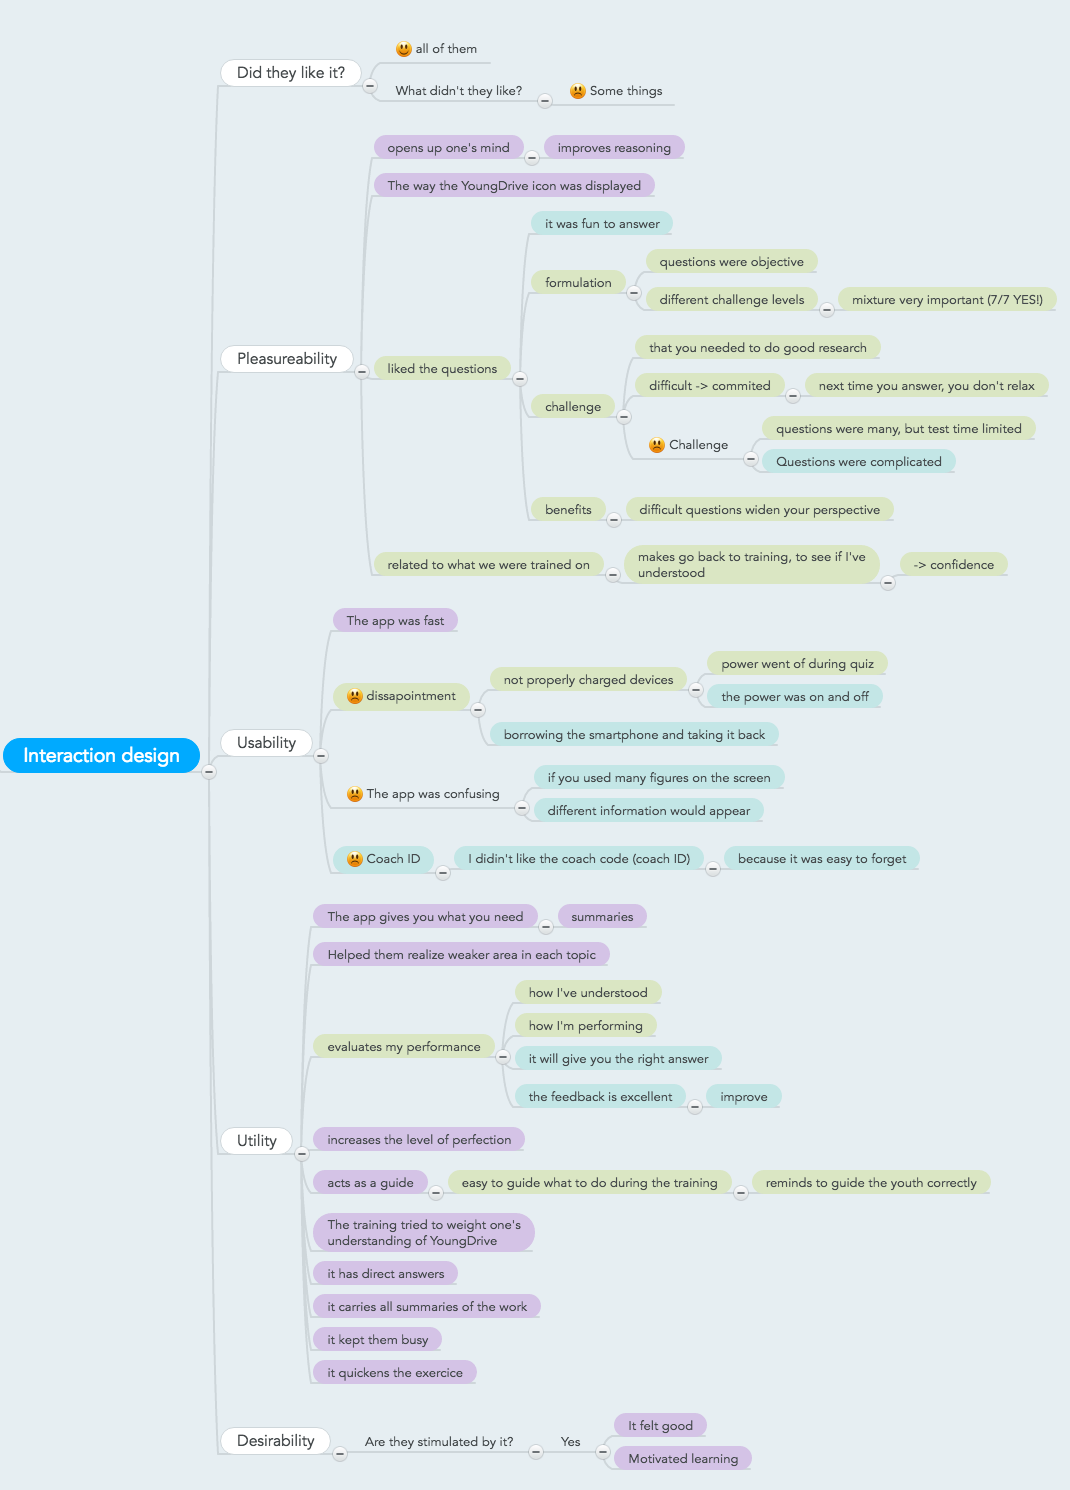
\includegraphics[width=1.0\textwidth]{iteration4qualitative_interactiondesign.png}
    \caption{Coach comments interaction design}
    \label{fig:interactiondesign}
\end{figure}

\begin{figure}[h]
    \centering
    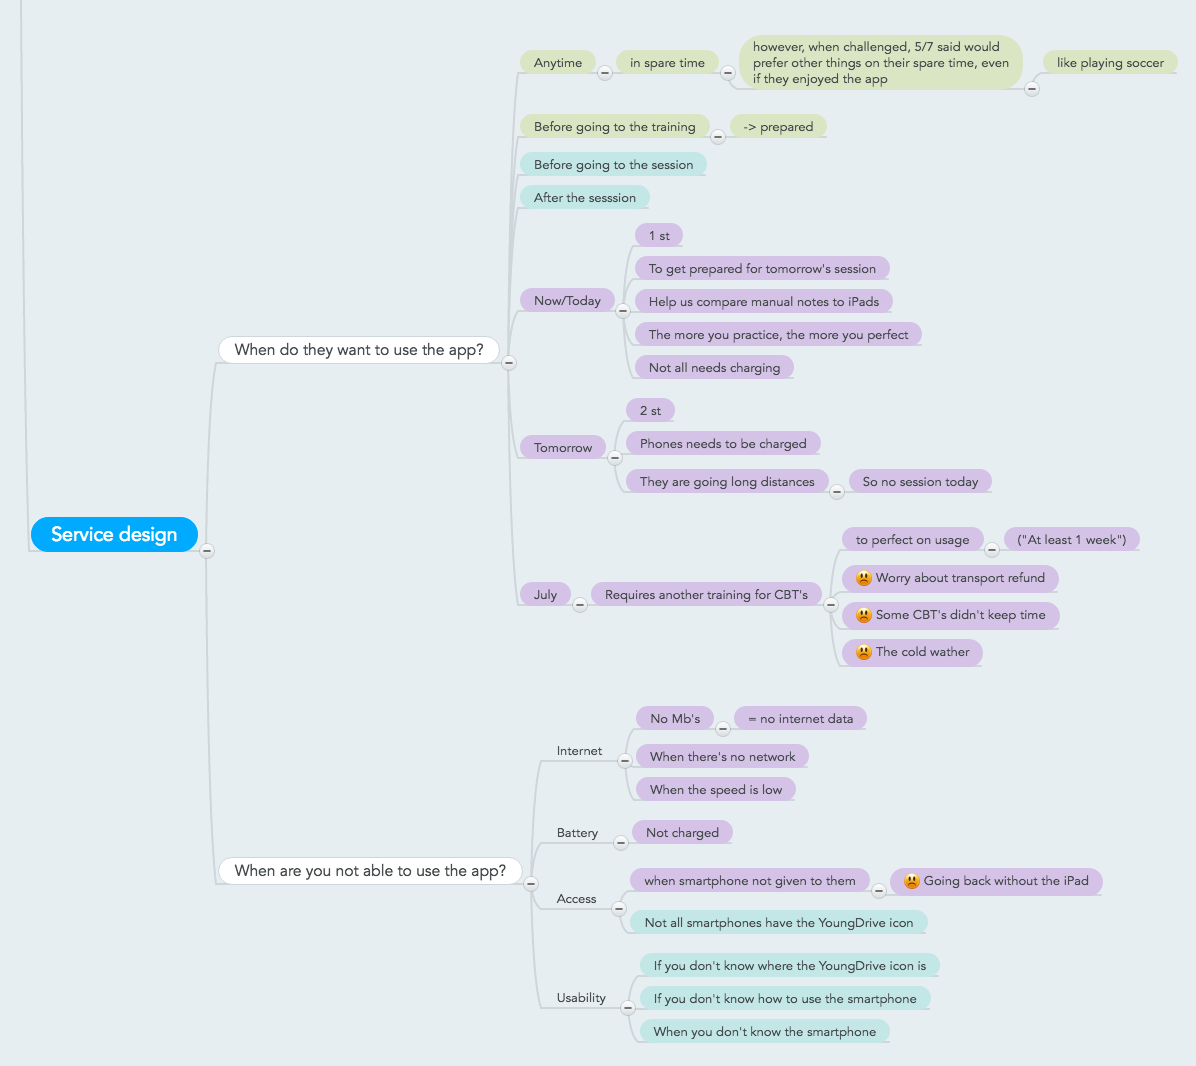
\includegraphics[width=1.0\textwidth]{iteration4qualitative_servicedesign.png}
    \caption{Coach comments regarding service design}
    \label{fig:servicedesign}
\end{figure}

\subsubsection{Test with the Plan Tororo staff}

With the Plan Tororo staff, it was shown how important the certification mode was: even though one group had 100\% on their first try, and a person had 1 wrong answer, the person with 1 wrong answer got 100\% on the certification, while the 100\% group had 1 wrong answer.

It is therefore determined, that when all of the answers can be answered correctly, after having gotten all answers correct once, that the knowledge is reliable - this is deliberate practice.
